\documentclass[11pt]{article}

% Packages
\usepackage[utf8]{inputenc}   % For UTF-8 encoding
\usepackage{amsmath, amssymb} % For mathematical symbols
\usepackage{graphicx}         % For including graphics
\usepackage{geometry}         % For adjusting page dimensions
\usepackage{hyperref}         % For hyperlinks
\usepackage{booktabs}         % For nicer tables
\usepackage{float}            % For figure placement

% Page layout
\geometry{a4paper, margin=1in}

% Document Info
\title{Model for U.S. Population Growth}
\author{Yijia Zhou}
\date{\today}

% Begin Document
\begin{document}

\maketitle


\section{Introduction}
This is a inventory model for the water and consumer demand based on the given data.

\section{Methods}
\subsection{Background}
The following data represent the number of gallons of water demand vs the number of occurrences (days). 

\begin{table}[H]
    \centering
    \begin{tabular}{ll}
        \toprule
        Number of Gallons Demanded & Number of Occurrences (Days) \\
        \midrule
        20 - 29 & 208 \\
        30 - 39 & 160 \\
        40 - 49 & 166 \\
        50 - 59 & 112 \\
        60 - 69 & 17 \\
        70 - 79 & 43 \\
        80 - 89 & 13 \\
        90 - 100 & 11 \\
        \bottomrule
    \end{tabular}
    \caption{Water demand data}
\end{table}


\subsection{Basic Simulatio Model}
Based on the original data, I created a histogram to visualize the probability distribution of the demand.

\begin{figure}[H]
    \centering
    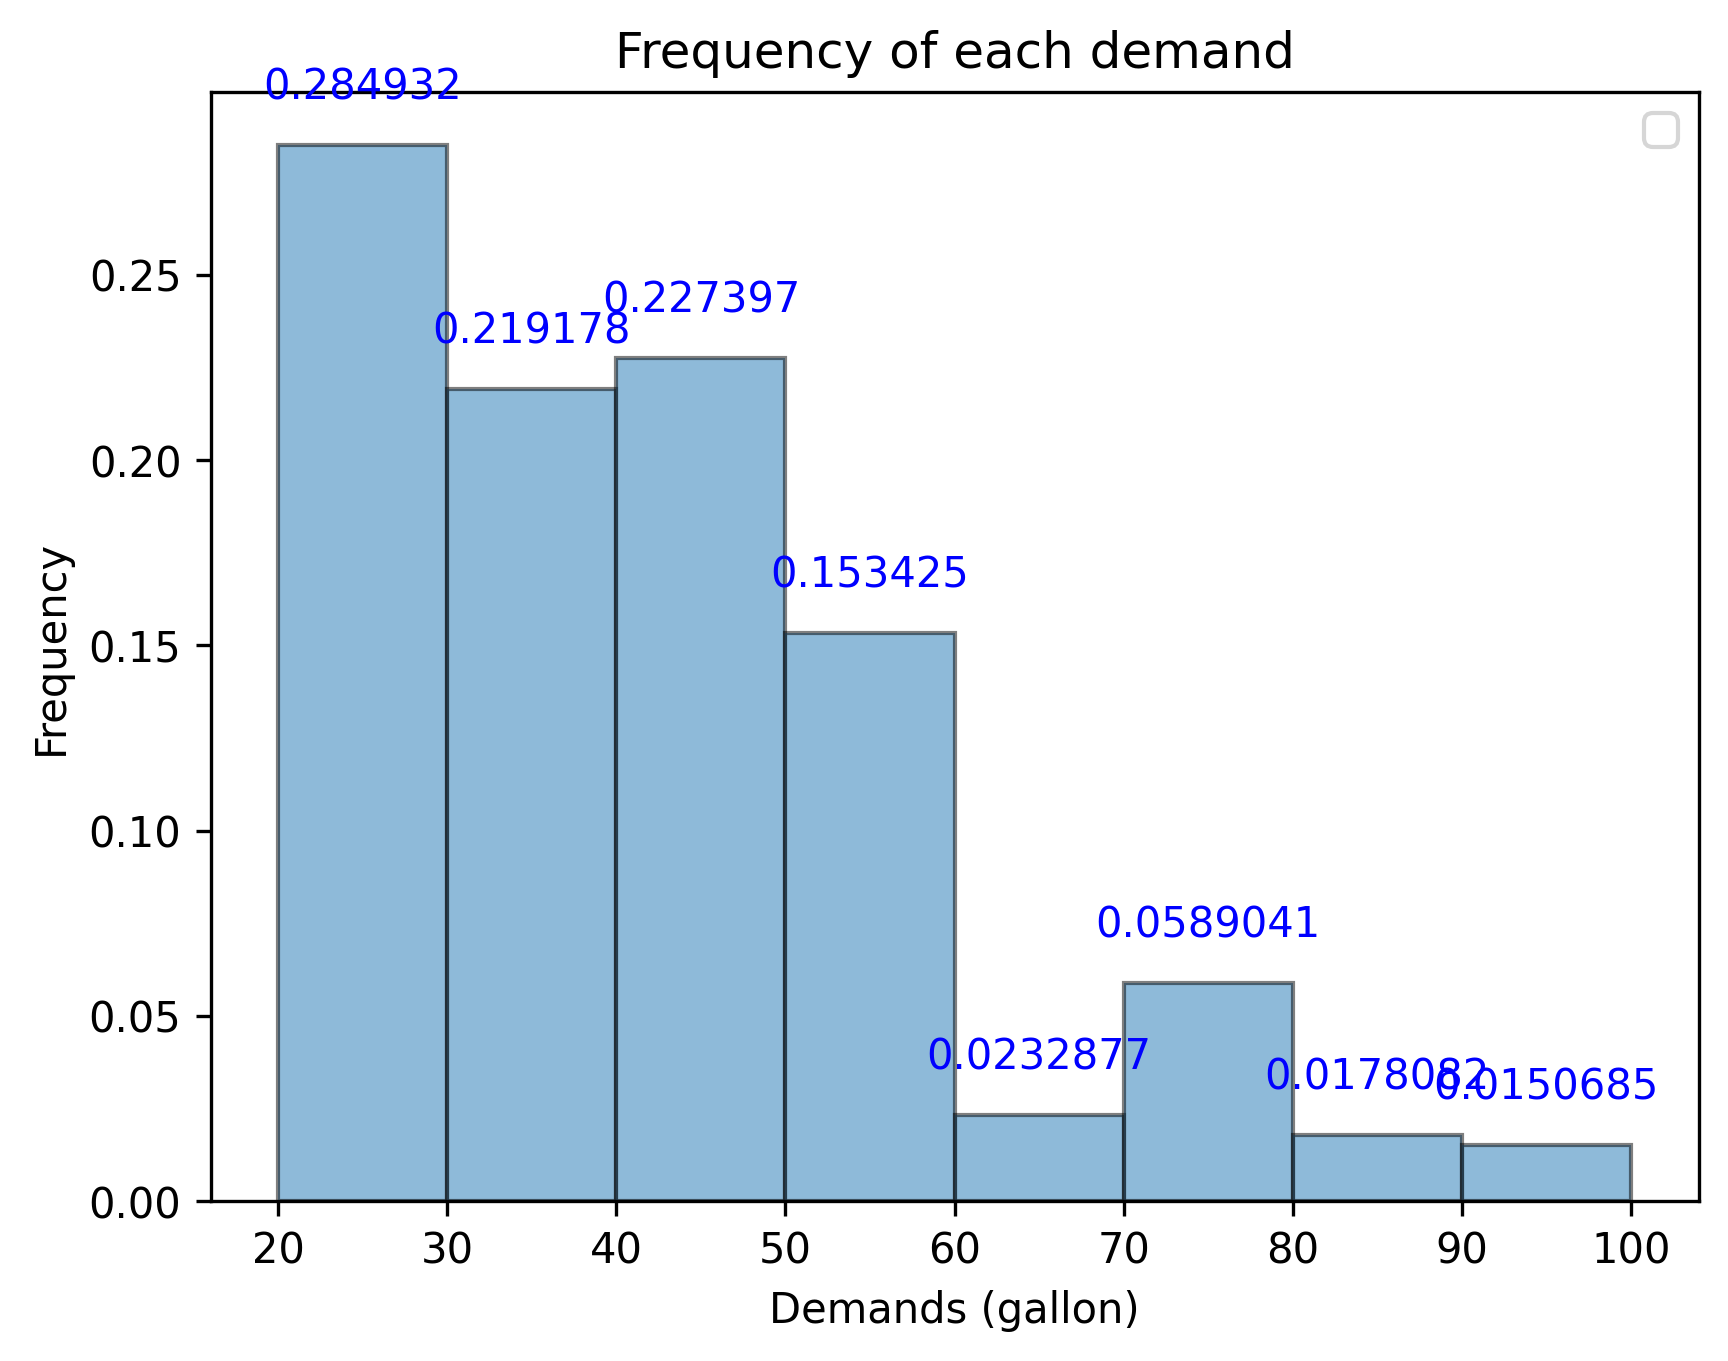
\includegraphics[width=0.5\textwidth]{histogram}
    \caption{Histogram of water demand probability distribution}
    \label{histogram}
\end{figure}


\subsection{Cumulative Probability Distribution}
Once we have the probability distribution, we can calculate the cumulative probability distribution. For simplicity, I assume the linear splines for each interval between two data points as shown in the figure.

\begin{figure}[H]
    \centering
    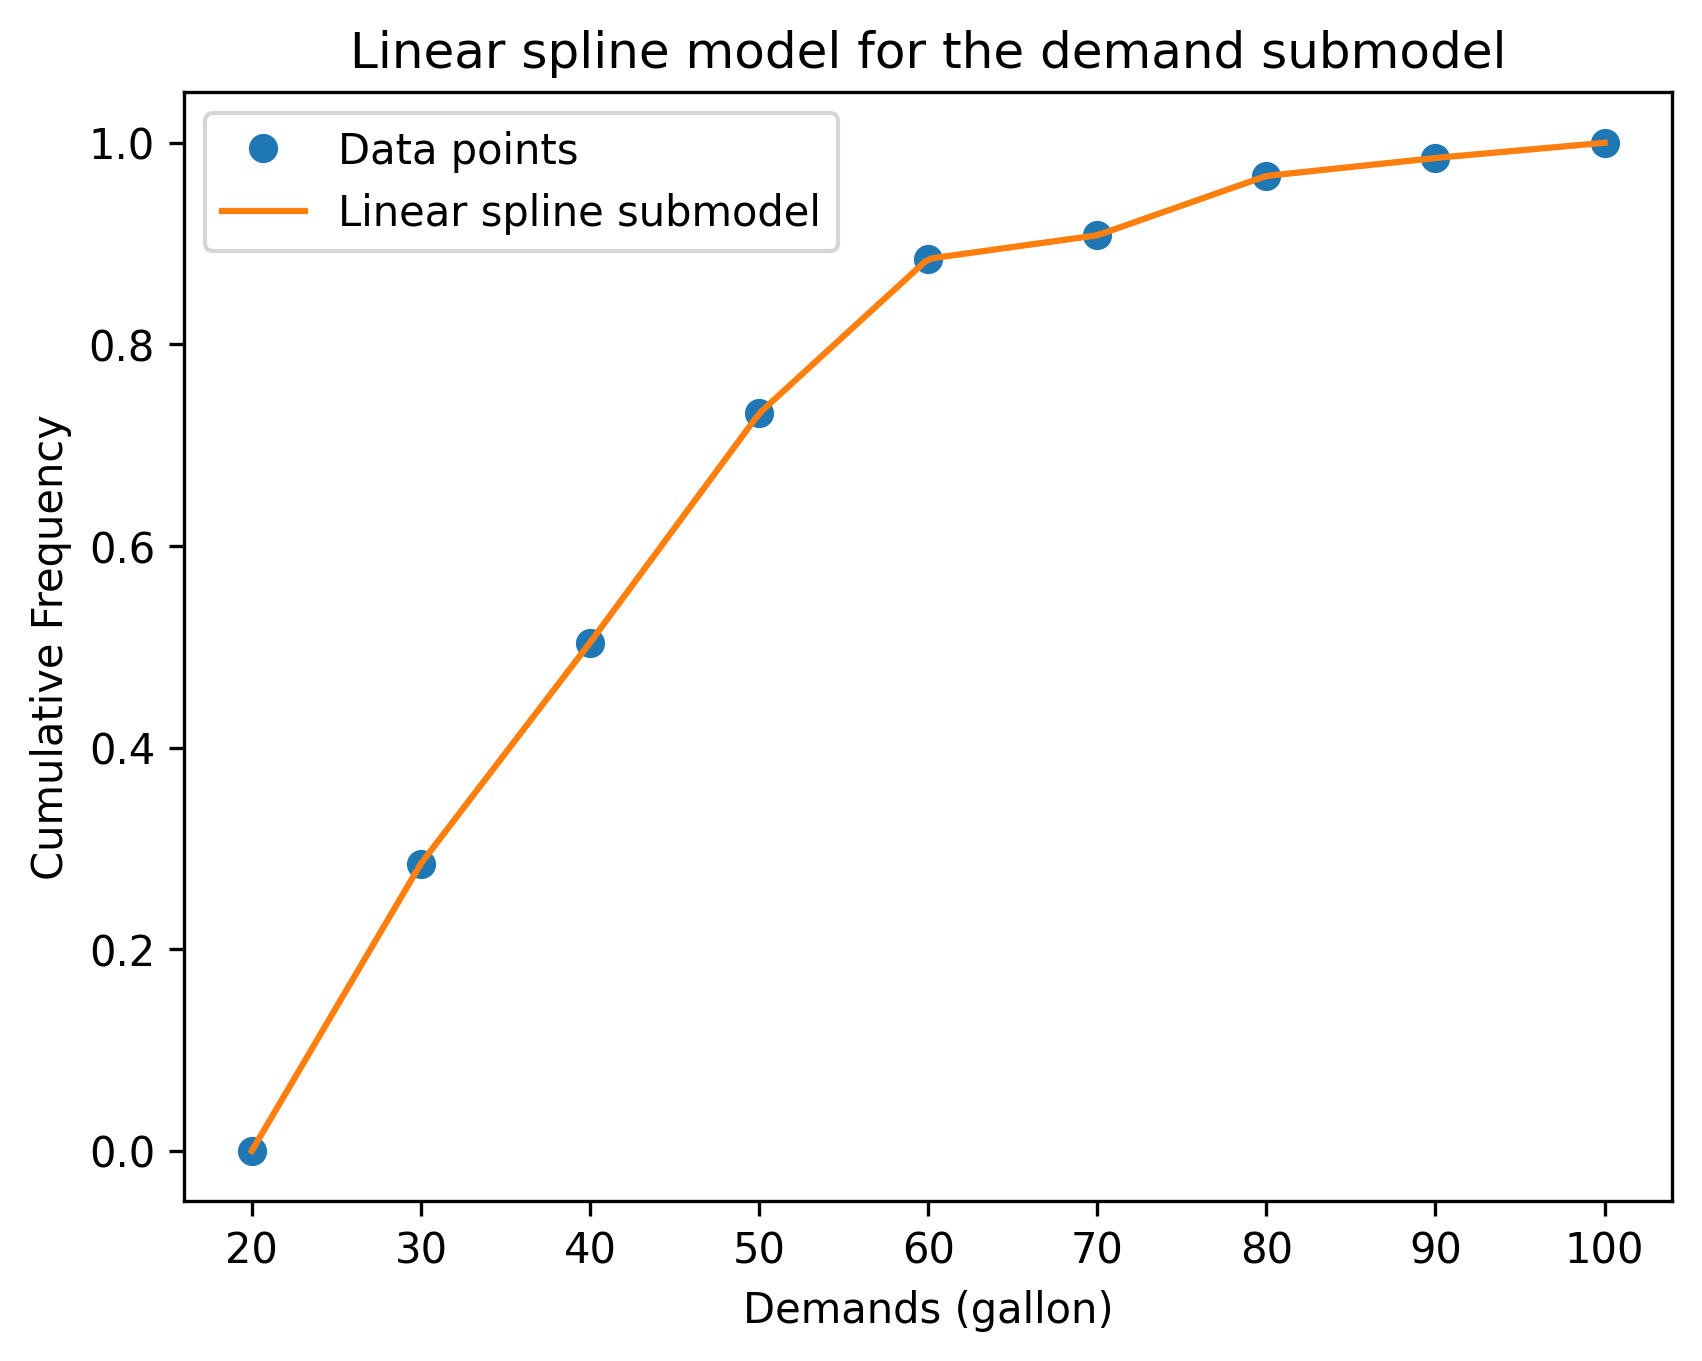
\includegraphics[width=0.5\textwidth]{interpolation}
    \caption{A linear spline model for the demand submodel}
    \label{fit}
\end{figure}

\subsection{Monte Carlo Inventory Algorithm}
Using the cumulative probability distribution, we can get a average cost histogram by running a Monte Carlo simulation 1000 times. The following parameters are used in the simulation:
\begin{itemize}
    \item Delivery Quantity Q = 800 gallons
    \item Time between deliveries T = 15 days
    \item Total length of simulation N = 365 days
    \item Delivery cost d = \$ 92.00 per delivery
    \item Storage cost s = \$ 0.001 per gallon per day
\end{itemize}

Using median demand (35 gallons) and average demand (42.34 gallons) as the basic test cases, we can get the average cost per day as 10.03 and 8.69 respectively.

\begin{figure}[H]
    \centering
    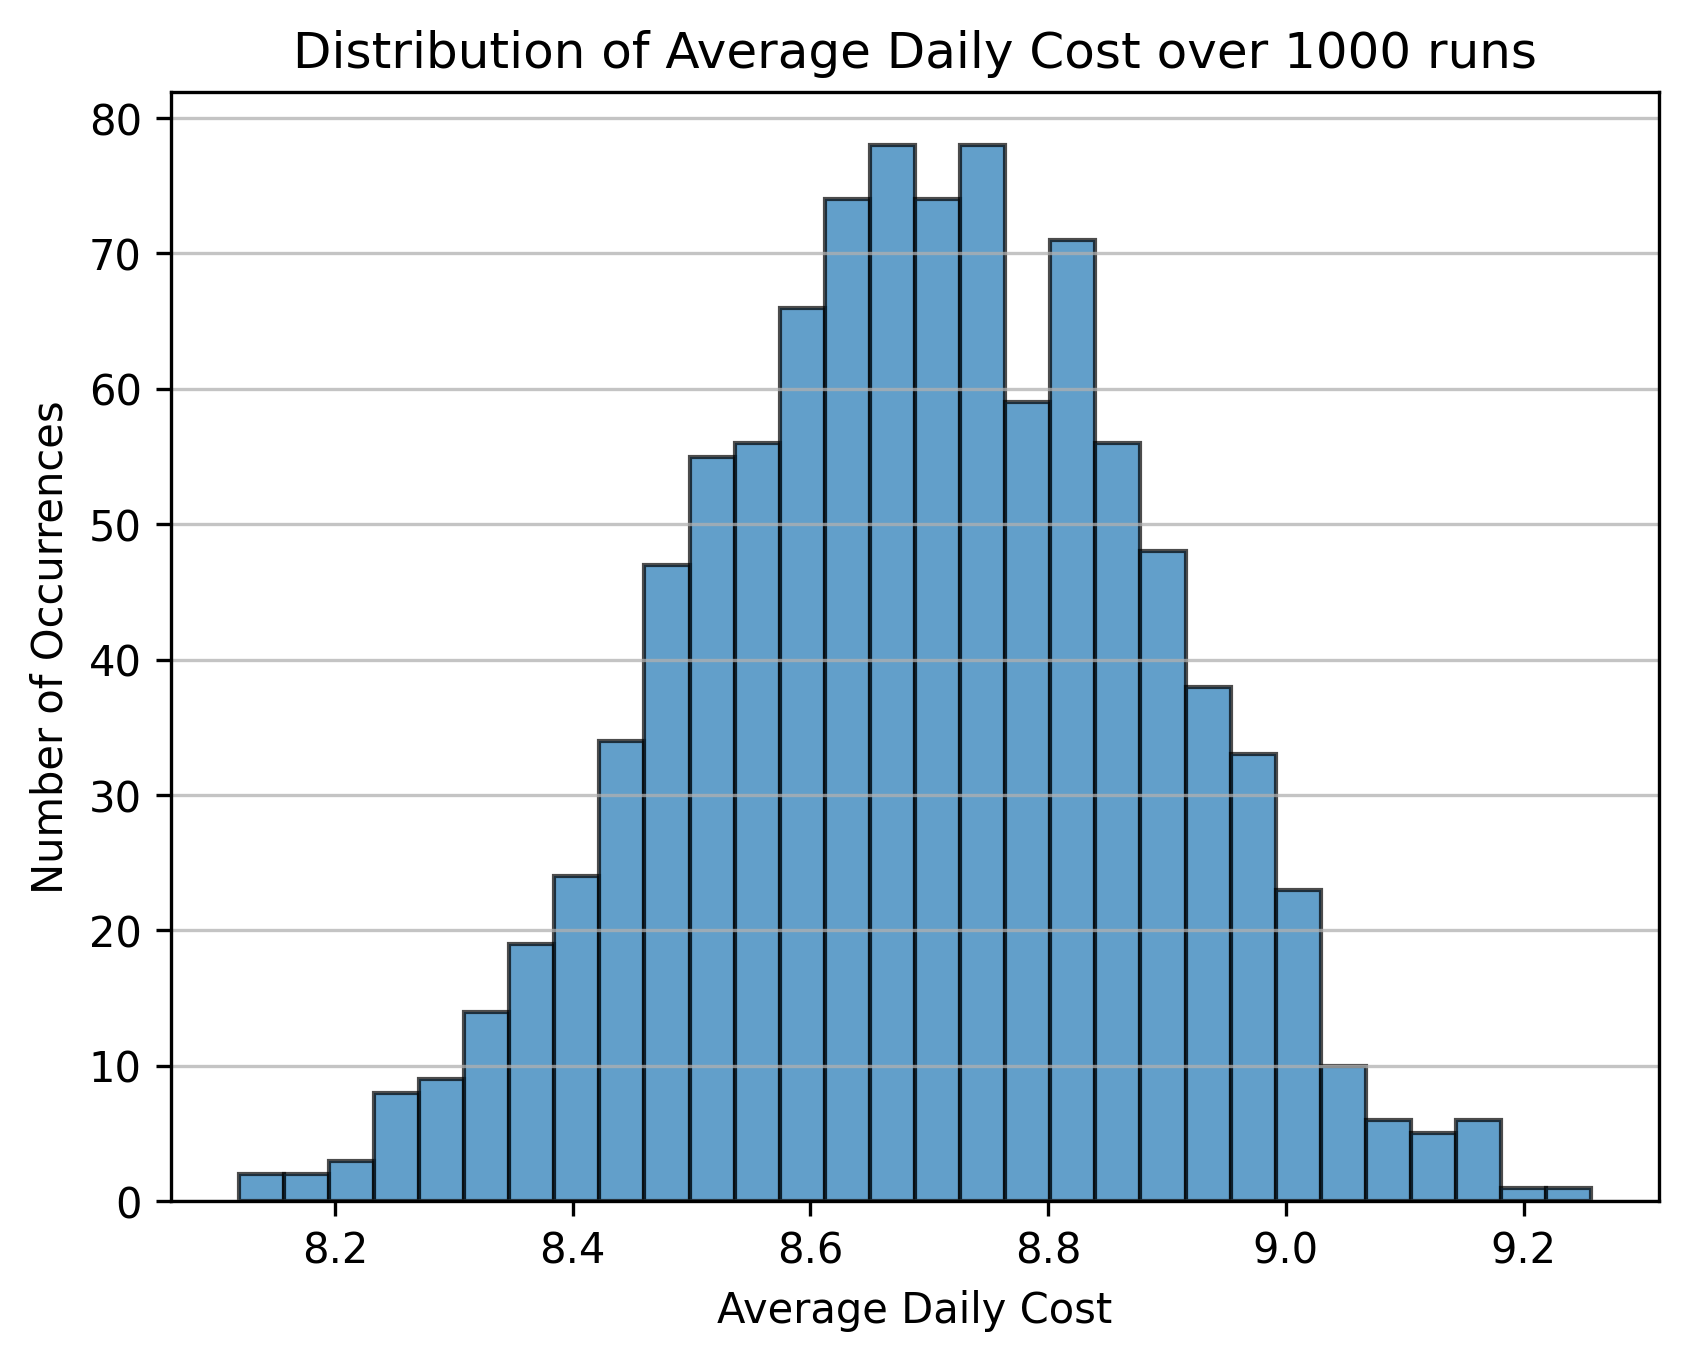
\includegraphics[width=0.5\textwidth]{cost_histogram}
    \caption{Histogram of average cost per day from Monte Carlo simulation}
    \label{average_cost}
\end{figure}

\section{Conclusion}
I created a basic inventory model based on the given data. The model can be further improved by using more sophisticated interpolation methods or by incorporating additional factors into the simulation.

\end{document}